
%%%%%%%%%%%%%%%%%%%%%%%%%%%%%%%%%%%%%%%%%%%%%%%%%%%%%%
\section{Evaluation} \label{sec:evaluation}

This section describes the evaluation of Iroko using our testbed built on the
Mininet simulator. The main goal is to compare the performance against the
existing centralized and decentralized techniques like Hedera~\cite{hedera} and
DCTCP~\cite{dctcp}.

\subsection{Benchmark suite}

For evaluation purposes, we are targeting a small scale data center of 16 hosts
and 20 switches with a FatTree topology. We take measurements for Hedera, DCTCP,
ECMP and a non-blocking switch on the same test setup. We consider the ECMP measurement
to be the base line. The non-blocking result represents a hypothetical single switch with full
backplane bandwidth, and is considered the theoretically achievable maximum. 

For traffic simulation, we use the same traffic matrices used in
Hedera~\cite{hedera}. We measured the following 3
traffic patterns:

\begin{enumerate} \item Stride$\left(i\right)$: A host with index $x$ sends to
the host with index $(x + i)mod(num hosts)$.  \item Staggered Prob $\left(EdgeP,
PodP\right)$: A host sends to another host on the same edge switch with
probability $EdgeP$, and to its same pod with probability $PodP$, and to the
rest of the network with probability $1-EdgeP - PodP$.  \item Random: A host
sends to any other host in the	network with uniform probability. We include
bijective mappings and ones where hotspots are present.  \end{enumerate}

Since we are primarily concerned about reducing the latency and packet drops
while keeping utilization at maximum, we measured bisection bandwidth and
    average queue length on the switches. The experiments lasted for 60 seconds for
    each benchmark and we consider only the middle 40 seconds.

\subsection{Bisection Bandwidth}

\begin{figure*}
	\centering
	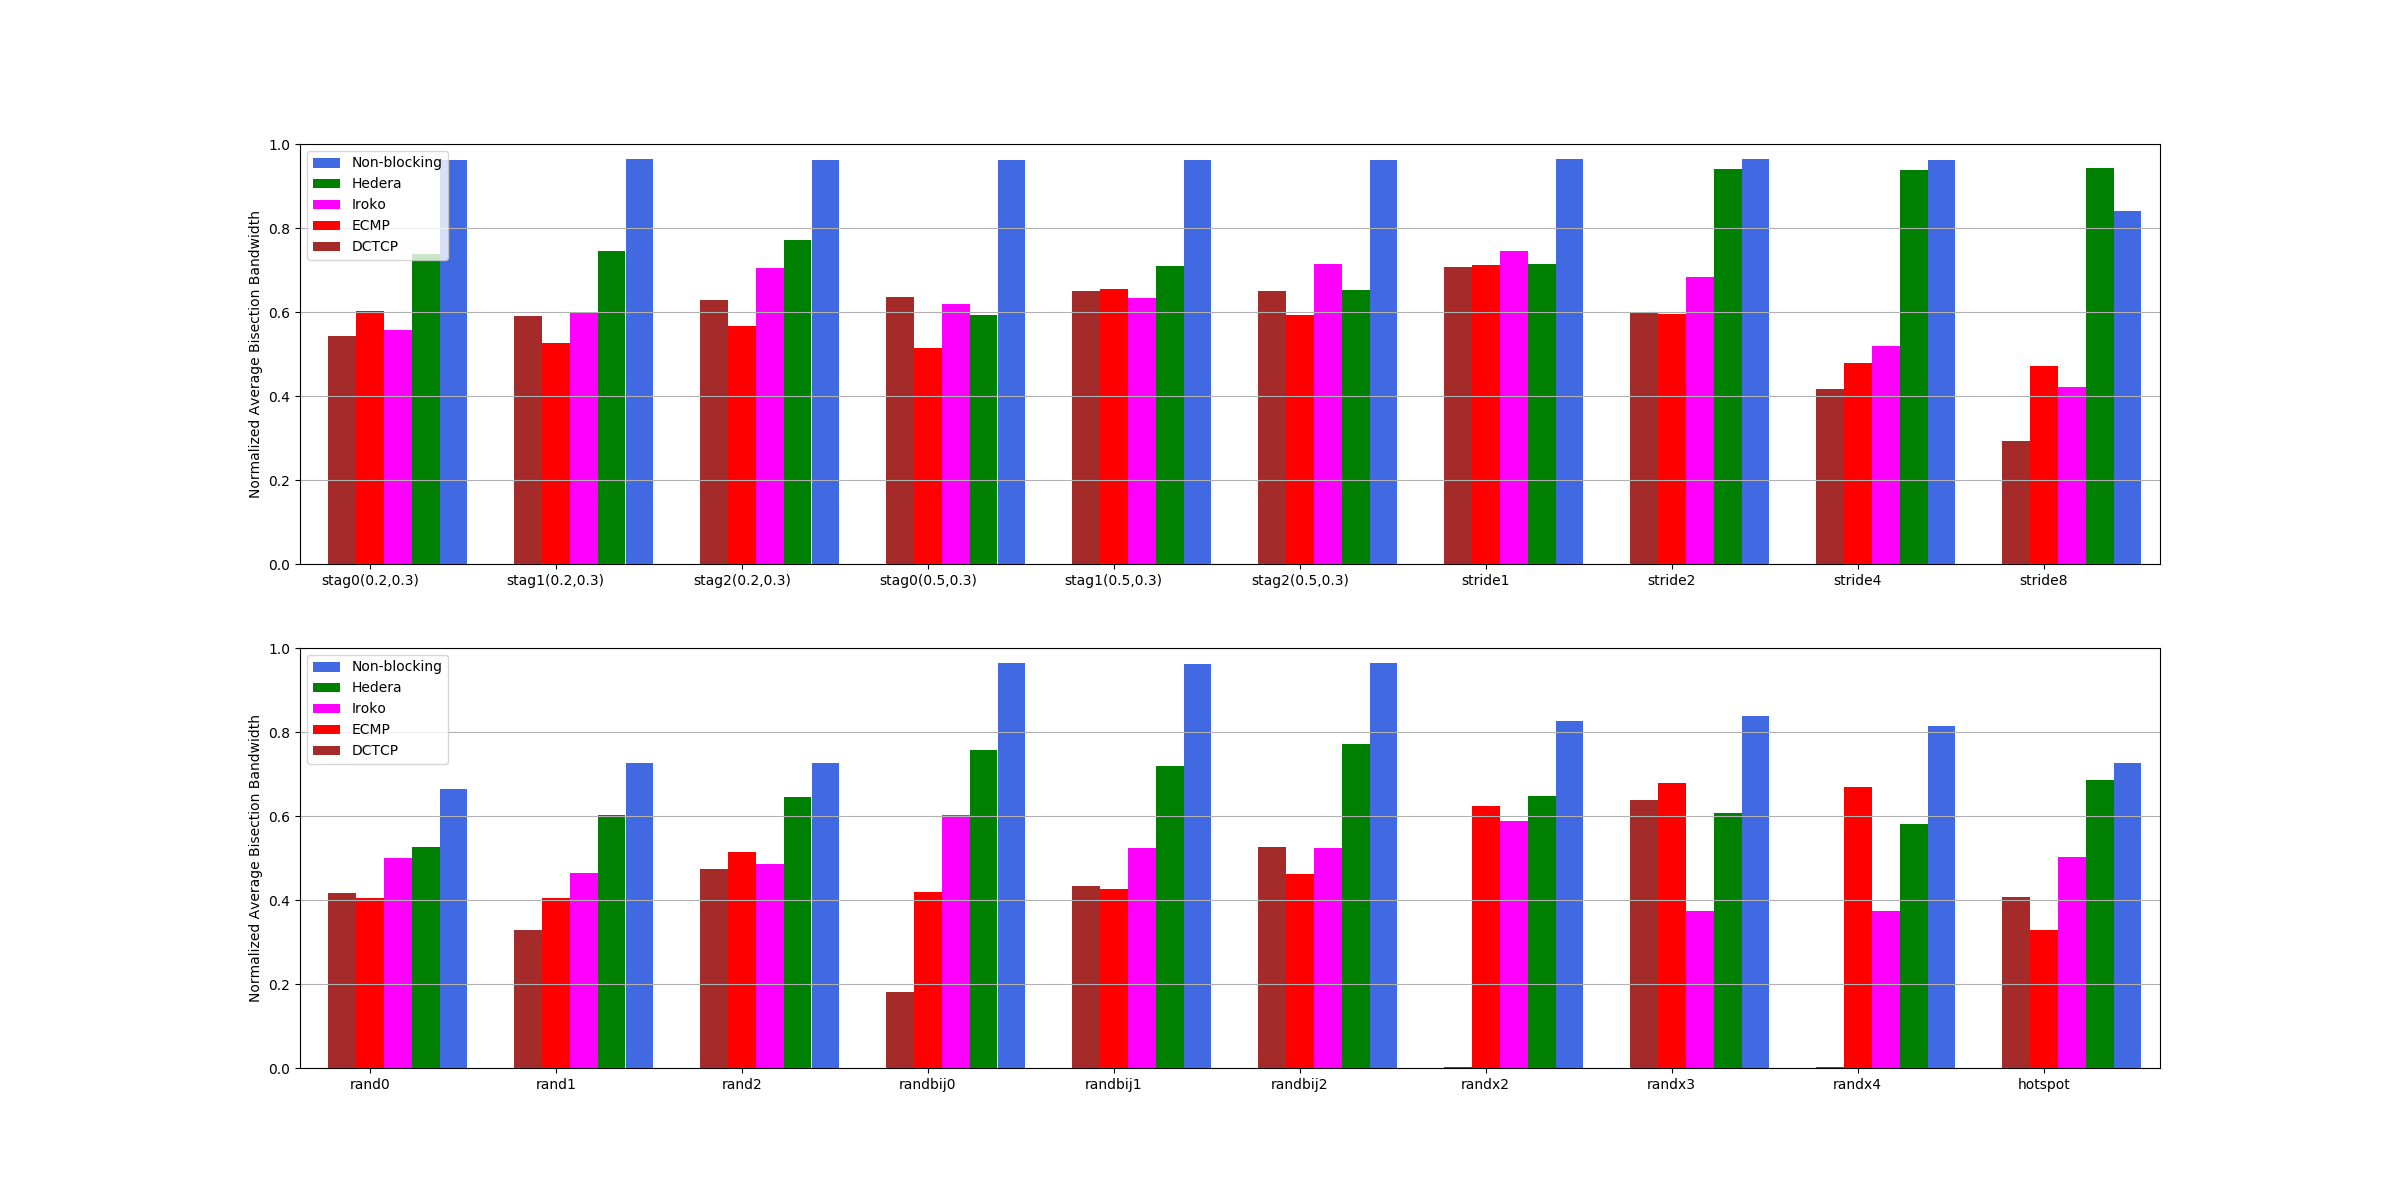
\includegraphics[width=1\linewidth]{rate.png}
	\caption{Average bisection bandwidth}
	\label{fig:rate}
\end{figure*}

In Figure \ref{fig:rate} we show the aggregate bisection bandwidth. Iroko
consistently provides better utilization compared to ECMP and DCTCP in almost
all experiments. As expected, non-blocking is providing the best performance out
of all four techniques. Utilization of non-blocking is lower for traffic
patterns with high incast. Hedera performs extremely well in all experiments
except for a few like stride1, stag2$(0.5,0.3)$ where Iroko outperforms Hedera.
Interestingly enough, Hedera even outperforms non-blocking in the stride8
experiment. ECMP does reasonably well when there is high probability of local
communication; for example smaller strides, but starts to deteriorate as the
stride length increases because of hash collisions.

Another interesting observation is that DCTCP gives abysmal utilization for some
experiments, for example, randx2 and randx4. Further investigation into this
revealed that this is because of DCTCP's aggressive congestion window size
reduction strategy on incast. The proposed solution for incast problems is to use
dynamic buffer allocation in switches, which is not implemented in our test
setup. General performance of DCTCP is not satisfactory either. For some
experiments it even under-performs ECMP.  According to the DCTCP paper, it is
optimized for some specific data center traffic patterns like web search, soft
real-time applications, recommendation systems etc., which we don't include in our
experiments.

\subsection{Drop rate}

\begin{figure*}
	\centering
	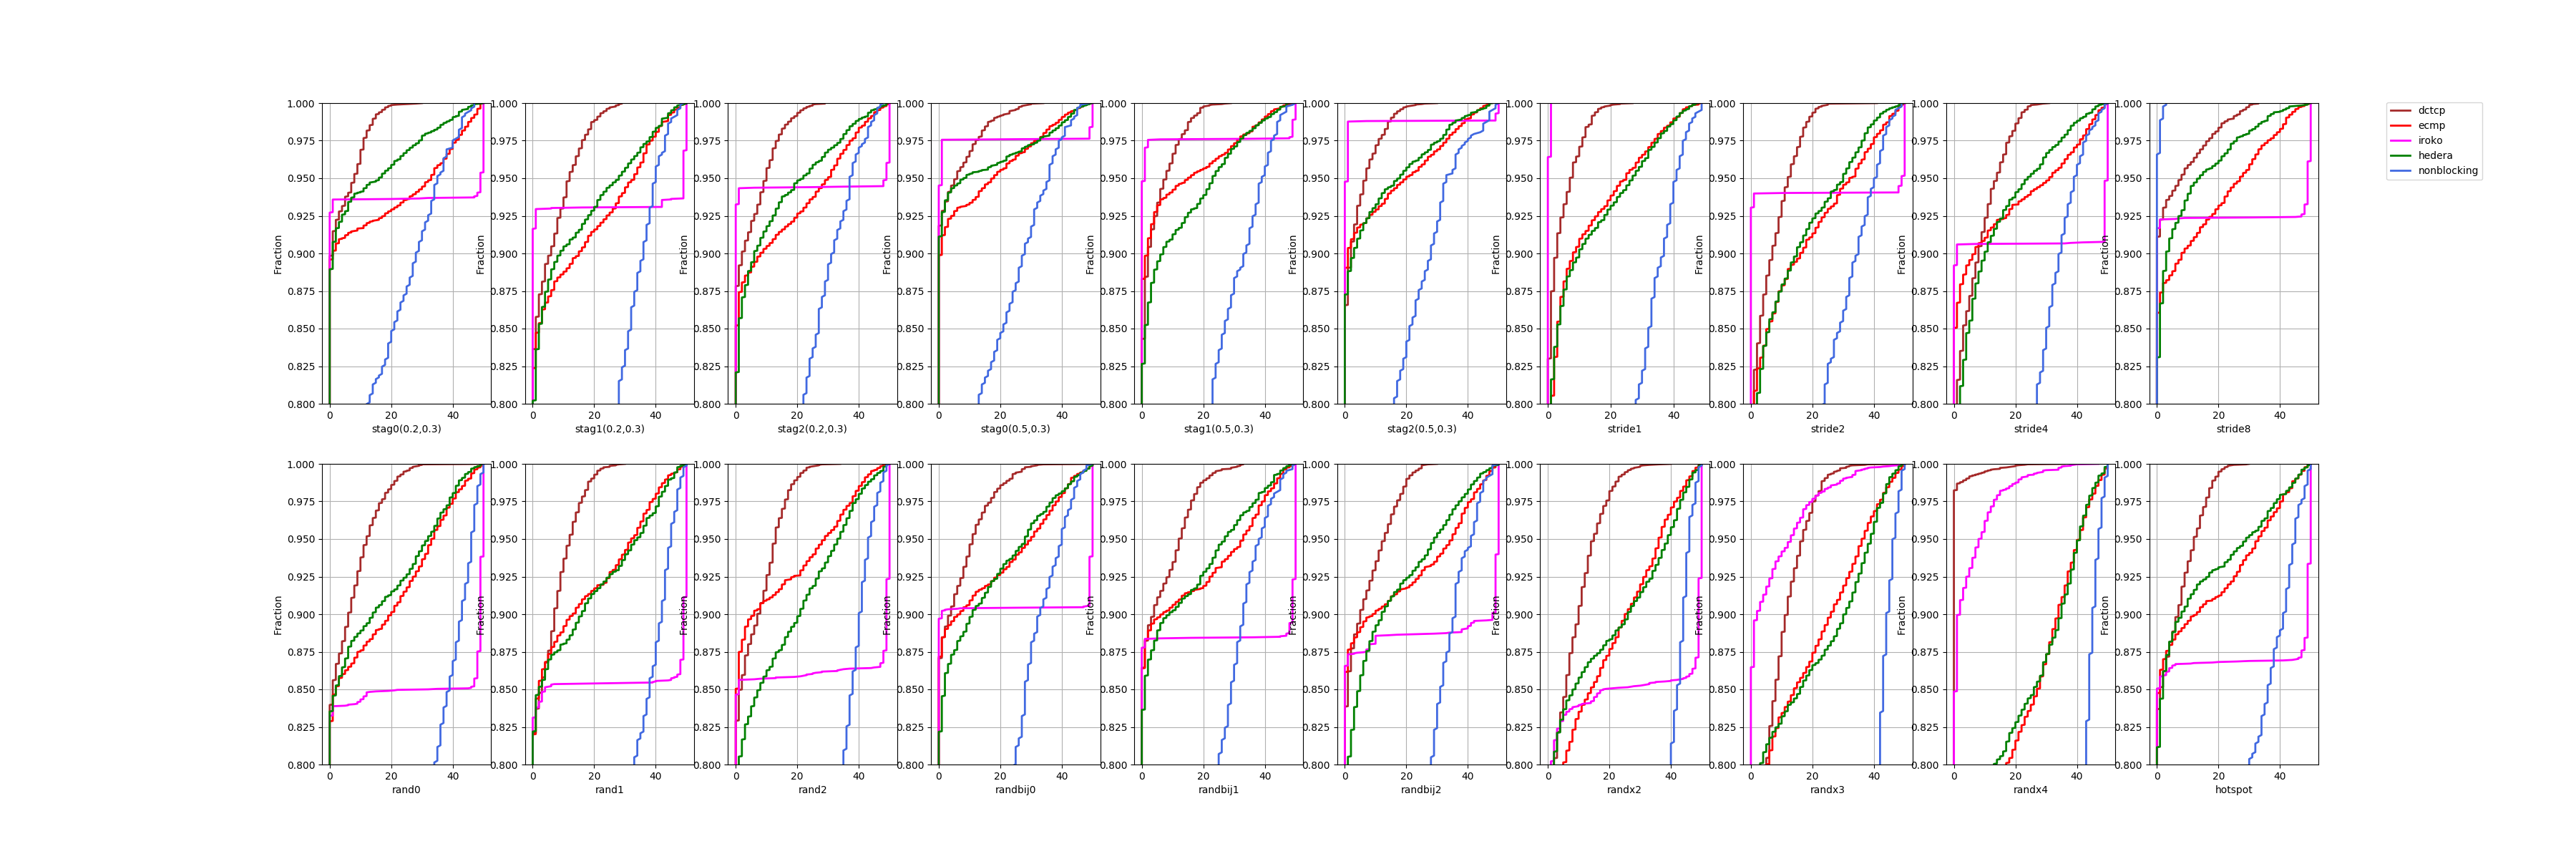
\includegraphics[width=1\linewidth]{qlen.png}
	\caption{CDF of queue lengths}
	\label{fig:qlen}
\end{figure*}

To analyze the drop rate we measured the number of packets built up in the queue
on all switches for the same set of traffic patterns and plotted a cumulative
distribution graph. In Figure \ref{fig:qlen} shows some selected
graphs. Recall that higher queue utilization is considered less optimal. For our experiments, we fixed the maximum
queue size at 50 packets.

Iroko struggles with queue management; consistently keeping $90\%$ of the queues
empty while the remaining $10\%$ are full. It is worth noting however, that Iroko performs
very well for traffic patterns like stride1, stag2$(0.5,0.3)$ etc., where it
shows high utilization. DCTCP maintains the queues at a minimum across
all experiments. This is not surprising considering the low utilization of
DCTCP. ECMP and Hedera behave almost the same. Non-blocking has the highest
queue size out of all techniques. We surmise that the CPU is the bottleneck here;
non-blocking uses only a single switch to connect the entire network with full
backplane bandwidth.

Iroko could definitely benefit from more fine tuning for the prediction algorithm. We further
need to investigate why the CDF of queue lengths exhibits a sudden jump from $0$ to $50$. Initial
analysis shows that a small fixed set of switches are the bottleneck in all
experiments. Our guess is that this happens because of the unfair bandwidth
allocation across traffic flows. Analyzing fairness might provide better insight
into this problem.

\subsection{More Benchmarks}

Apart from utilization and loss rate, the following benchmarks remain of interest.
Due to time constraints, we were not able to fully investigate these.

\begin{enumerate}

\item \textbf{99th percentile latency:} We are aiming for a low latency solution,
which means that the 99th percentile latency in the network across all flows should
be as low as possible.

\item \textbf{Fairness:} Fairness across flows can be tested by introducing a
new host to a completely saturated network and increasing the transmission rate
to see if all the hosts gets fair share of the total bandwidth. Currently we are
assuming that all flows should be given equal priority. Differential priority is out of
scope.

\item \textbf{Responsiveness:} This metric evaluates the predictive power and
efficiency of Iroko. It would be interesting to analyze the response time of the
central scheduler compared to decentralized DCTCP and TCP.

\item \textbf{Starvation:} Since we are rate limiting at the host level, Iroko
should make sure that no flows are starving to send data. This can be measured
by plotting residual bandwidth and excess load.

\end{enumerate}
